% last updated in April 2002 by Antje Endemann
% Based on CVPR 07 and LNCS, with modifications by DAF, AZ and elle, 2008 and AA, 2010, and CC, 2011; TT, 2014

\documentclass[runningheads]{llncs}
\usepackage{graphicx}
\usepackage{amsmath,amssymb} % define this before the line numbering.
\usepackage{ruler}
\usepackage{color}
\usepackage{array}
\usepackage{float}
\usepackage{subfig,caption}
%\usepackage{subcaption}
\usepackage{comment}
\usepackage[width=122mm,left=12mm,paperwidth=146mm,height=193mm,top=12mm,paperheight=217mm]{geometry}
\begin{document}
% \renewcommand\thelinenumber{\color[rgb]{0.2,0.5,0.8}\normalfont\sffamily\scriptsize\arabic{linenumber}\color[rgb]{0,0,0}}
% \renewcommand\makeLineNumber {\hss\thelinenumber\ \hspace{6mm} \rlap{\hskip\textwidth\ \hspace{6.5mm}\thelinenumber}}
% \linenumbers
\pagestyle{headings}
\mainmatter
\def\ECCV14SubNumber{***}  % Insert your submission number here

\title{Author Guidelines for ECCV Submission} % Replace with your title

\titlerunning{ECCV-14 submission ID \ECCV14SubNumber}

\authorrunning{ECCV-14 submission ID \ECCV14SubNumber}

\author{Anonymous ECCV submission}
\institute{Paper ID \ECCV14SubNumber}


\maketitle

\begin{abstract}

\end{abstract}


\section{Introduction}
Features learnt by a large-scale convolutional neural network trained for the task of image classification on the Imagenet challenge have been used to achieve impressive results on different computer vision tasks. Since, these networks are high capacity learners they cannot be trained on small data sets. Consequently, in their recent work ..have used fine-tuning to improve performance. For example, (\cite RCNN) used fine-tuning to boost performance on pascal detection challenge by nearly 25 \% (relative) mean ap points over the performance of an un-tuned network.

Fine-tuning a network essentially involves starting from a set of pre-learned parameters and slowly updating them to minimize a target loss function. Till date, there has been little work looking at the effect of fine-tuning on various layers of a discriminatively trained convolutional neural network. In this work, we address this question. Our findings indicate that during finetuning most of the learning takes place in the top 2 fully connected layers whereas the convolutional layers are largely un-changed. We quantify this claim by first comparing entropy of filters before and after fine-tuning. Secondly, we demonstrate that keeping layers 1-5 fixed while fine-tuning leads to negligible decrease in performance. Next, we show pool-5 features can be treated as generic feature extractor on top of which non-linear classifiers can be used to achieve good results. For developing a scientific understanding of how the network trains, we analyse conv-nets trained for different number of iterations. We find that most of the learning happens quite early on and that the network naturally learns in a layer-wise fashion. Finally, we conclude by providing some insights into how important is the magnitude of feature activation, the location and so on. 

This suggests, that layers 1-5 can be treated as a generic feature extraction engine which can serve as a starting point for other computer vision models. Reduce time for fine-tuning. 
The most commonly used conv-net architecture, first proposed by Kr consists of 5 convolutional layers followed by 2 fully connected layer. 
 
Inspite of the impressive performance, the question of how information is represented and what various layers are encoding is unclear. 

Some recent work has focussed on coming up with visualization techniques to analyze and understand the tuning properties of filters in different layers. Although, visually impressive its hard to draw meaningful conclusions about properties of filters in different layers. We start of f with a detailed analysis of how good are different layers for image classification. We provide an entropy analysis ...

Next, we try to answer how much information is encoded by the activity of individual filters and how important is the spatial location of where the filters activate.      

Next, we show that the network trains layer-wise and the convolutional layers are well formed quite early into the training. 

Next, we argue that fine-tuning majorly effects the final two layers and that layers 1-5 can be treated as a generic feature extractor. This allows us a moderate speed-up in training time. 

\section{Relevant Work}

\section{Method}
\subsection{Network-Architecture}
For all our experiments we closely follow the architecture proposed in \cite{alex}. The first 2 layers consist of 4 sublayers each - convolution (conv), followed by rectified linear units (relu), pooling (pool) and contrast normalization (norm). Layers 3, 4 are composed of convolutional units followed by relu units. Layer 5 consists of convolutional units, followed by relu and pooling. The last two layers are fully connected (fc). In this work when we refer to a layer without referring to a particular sub-layer - then for layer 1,2,5 we mean the output of the pooling stage and for layers 3,4,6,7 we mean the output of relu units.

\subsection{Training Conv-Nets}
We have trained all our models using the publically available code \cite{caffe} and Nvidia K40 GPUs. Our imagenet network was trained for 310000 iterations and achieves an error rate only about 2\% higher on the ILSVRC validation set 2012. We refer to this network as the Alex-net .

\subsection{Fine-Tuning}
For a particular task, we fine-tune conv-nets by running SGD (Stochastic Gradient) with a starting learning rate set to $\frac{1}{10}^{th}$ of the intial learning rate of the imagenet model. This choice has been made because we donot want to drastically change the parameters of the network and overfit to the training set. At every 20,000 iterations we reduce the learning rate by a factor of 10 and use a mini-batch size of 128.

\subsubsection{Fine-Tuning for PASCAL}: Closely following the work of \cite{rcnn} we use region proposals generated by selective search algorithm for fine-tuning. Each region is warped to a size of 227*227*3. Regions with IOU (intersection over union) $\geq$ 0.5 with ground truth bounding boxes are treated as positives and rest as negatives. This  results into a 21-way classification problem (20 PASCAL classes + background). We tuned this network for 70000 iterations and refer to it as the FT network in the sections below.

**To-DO ? Specify the procees of fc-only fine-tuning.  ***

\section{Discriminative Pre-Training + Fine-Tuning Helps}
**To-Do** Results on SUN


\setlength{\tabcolsep}{2pt}
\begin{table}
\begin{center}
\caption{Effect of fine-tuning a network for 3 tasks in the PASCAL VOC-2007 Challenge}
\label{table:fine-effect}
\begin{tabular}{l|ccc|ccc|ccc}
\hline\noalign{\smallskip}
Layer & \multicolumn{3}{c}{Image Classification}  & \multicolumn{3}{c}{GT Box Classification} & \multicolumn{3}{c}{Detection} \\
\hline
      & alex-net & fc-tune & all-tune & alex-net & fc-tune & all-tune & alex-net & fc-tune & all-tune \\
\hline
pool-5   & 65.6 & & 64.6 & 79.1 & 79.1 & 79.5 & 45.0 & 45.0 & 47.6 \\
relu-6   & 70.6 & & 71.7 & 79.4 & 82.0 & 82.3 &  - & 51.0 & 53.1  \\
relu-7   & 73.6 & & 73.2 & 79.9 & 83.4 & 85.2  & 45.5 & 53.3 & 54.1 \\
\hline
\end{tabular}
\end{center}
\end{table}
\setlength{\tabcolsep}{1.4pt}



\subsection{Layer-Wise Effect of Fine-Tuning}

\setlength{\tabcolsep}{4pt}
\begin{table}
\begin{center}
\caption{Layerwise effect of fine-tuning, GT-bbox classification, FT: Fine-Tuned, C-Net: Caffe-Net}
\label{table:headings}
\begin{tabular}{ccc|ccc|ccc|ccc}
\hline\noalign{\smallskip}
Layer & C-Net & FT & Layer & C-Net & FT & Layer & C-Net & FT & Layer & C-Net & FT \\
\noalign{\smallskip}
\hline
\noalign{\smallskip}
l1 & 43.2 & 43.2 & l3 & 73.3 & 73.7 & l5 & 79.1 & 79.5 & \textbf{l7} & \textbf{79.9} & \textbf{85.1} \\
l2 & 67.1 & 67.7 & l4 & 75.5 & 77.8 & \textbf{l6} & \textbf{79.4} & \textbf{82.3} \\
\hline
\end{tabular}
\end{center}
\end{table}
\setlength{\tabcolsep}{1.4pt}

**To-Do**: Difference in Entropy


\subsection{FC-Only Fine-Tuning is Sufficient}
We evaluated 3 convolutional neural networks (namely caffe-net, FT and FC-FT) on the tasks of image classification, ground truth bounding box classification and detection. The results can be seen in table \ref{table:fine-effect}. The mean-AP on the tasks of ground truth bounding box classification and detection increases, whereas performance is uneffected for the task of classification. The performance of the network with tuning the fully connected layers is comparable to the performance of


In order to test our hypothesis that bulk of the learning required for good performance on a new task happens in the fully connected (FC) layers - we finetune caffe-net in two ways. In the first method, we set the learning rate for all the convolutional layers to be zero and randomly intialize the fully connected layers. The second network has non-zero learning rates for all the layers and the FC-layer parameters are initialized to their values in a conv-net trained on imagenet. Fine-tuning is performed  using the selective search bounding box proposals (\cite{rcnn}). The ground truth bounding boxes are assigned their respective class labels whereas any region with less than 0.3 IOU with a ground truth bounding box is assigned to background class. We fine-tune both the networks for 70,000 iterations.

Results of this experiment are presented in table \ref{table:det-fine}. The full fine-tuned network does slightly better when we train a detector on pool-5 features but the performance after layer 7 is almost equal. 

\setlength{\tabcolsep}{1pt}
\begin{table}
\begin{center}
\caption{Detection: Fine-Tuning Effects.}
\label{table:det-fine}
\tiny
\begin{tabular}{l|cccccccccccccccccccc||c}
\hline\noalign{\smallskip}
Feature & aero & bike & bird & boat & bottle & bus & car & cat & chair & cow & table & dog & horse & mbike & person & plant & sheep & sofa & train & tv & mAP \\
\noalign{\smallskip}
\hline
l5 & 51.9 & 61.1 & 36.8 & 28.4 & 23.7 & 52.3 & 60.8 & 48.4 & 24.9 & 47.1 & 47.5 & 42.1 & 55.6 & 58.7 & 42.5 & 24.5 & 46.9 & 39.3 & 52.0 & 55.4 & 45.0 \\
l5-ft & 57.8 & 63.9 & 38.8 & 28.0 & 29.0&54.8&66.9&51.3 & 30.5 & 52.1 & 45.2 & 43.2 & 57.3 & 58.8 & 46.0 & 27.2 & 51.2 & 39.3 & 53.3 & 56.6 & 47.6 \\
\hline 
l6-ft &63.5 & 66.3 & 48.7 & 38.1 & 30.6 & 61.4 & 70.9 & 60.3 & 34.8 & 57.8 & 47.6 & 53.6 & 59.8 & 63.5 & 52.5 & 29.8 & 54.6 & 48.2 & 58.5 & 62.2 & 53.1 \\
l6-fc-ft& 61.4 & 63.9 & 44.2 & 36.2 & 29.0 & 59.9 & 66.0 & 55.3 & 31.1 & 57.6 & 49.5 & 49.4 & 59.4 & 63.7 & 50.8 & 29.5 & 54.1 & 43.2 & 57.4 & 58.8 & 51.0 \\
\hline
l7 & 57.6 & 57.2 & 41.4 & 31.2 & 25.6 & 52.4 & 58.8 & 50.9 & 25.2 & 50.4 & 42.7 & 47.1 & 52.2 & 55.6 & 44.5 & 23.9 & 48.0 & 38.1 & 51.5 & 56.6 & 45.5 \\
l7-ft & 64.3 & 69.6 & 50.1 & 41.8 & 32.0 & 62.6 & 71.0 & 60.6 & 32.8 & 58.5 & 46.4 & 56.0 & 60.0 & 66.9 & 54.2 & 31.5 & 52.7 & 48.8 & 57.7 & 64.7 & 54.1 \\
l7-fc-ft & 62.9 & 65.2 & 47.5 & 39.0 & 30.3 & 63.1 & 68.4 & 59.7 & 34.2 & 58.5 & 52.0 & 53.8 & 60.7 & 65.3 & 53.0 & 30.2 & 55.5 & 46.3 & 57.7 & 62.2 & 53.3 \\
\noalign{\smallskip}
\hline
\end{tabular}
\end{center}
\end{table}
\setlength{\tabcolsep}{1.4pt}


The performance of the FC-FT network at layer 5 is slighly worse by 2.6 points, but at layer 7 this difference is only 0.8 points. 

Next, we compare the performance of both the networks for the task of classifying ground-truth bounding boxes from PASCAL-VOC-2007 challenge.  

\subsection{Replacing fc-layers by other-non linear classifiers}
**Stacked Kernel Results ***


\section{Speed of Learning}
Convolutional neural networks take a long time to train. For achieving state of art accuracy on the imagenet challenge these networks are often trained on high-end GPUs for more than 7 days. Even our implementation of fine-tuning following the approach proposed in \cite{rcnn} takes more than 12 hours on a Nvidia Tesla-K40. A way to speed up training will allow for a rich exploration of network architectures and parameters which is currently not possible.    

As a first step towards addressing this problem, we looked at the evolution of training loss and validation accuracy as the training progresses (fig \ref{fig:conv1}.) The top-1 accuracy on the imagenet validation set at 15K iterations is at 29.5 \% and 38.13\% at 50K iterations (compared to 57.4 \% at 310K iterations). The training loss rapidly increases initially and then there is a slow sluggish decay except for the point where learning rate is decimated by a factor of 10 at 100K iterations.

The first thing we try to answer is - if there is an insightful intepretation of the fast intial drop in training loss. Towards this end, we visualized layer 1 filters at different time instances. Surprisingly, we found that within 15K iterations these filters look almost identical to what they would be by the end of the training (See fig \ref{fig:conv1}). This naturally leads us to ask the question what happens at other layers ? Also, since it is hard to train these massive networks from sratch on small data-sets and discriminative pre-training has been found to be helpful we would also like to understand if there exists a critical point by which the network learns all that there is in order to generalize.  

In order to answer these question and objectively assess the temporal evolution of quality of filters we measure classification performance of features extracted from individual layers on PASCAL-VOC-2007.  The results are summarized in table \ref{table:det-trajectory}. 

\begin{figure}
\centering
\subfloat{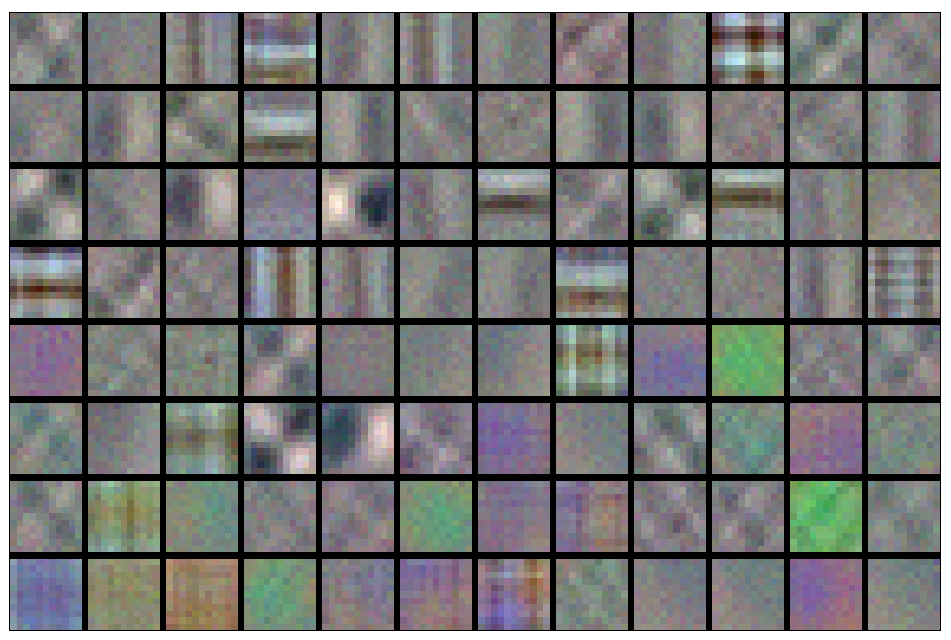
\includegraphics[scale=0.10]{images/l1_filters_iter5000.png}} \hspace{2mm}
\subfloat{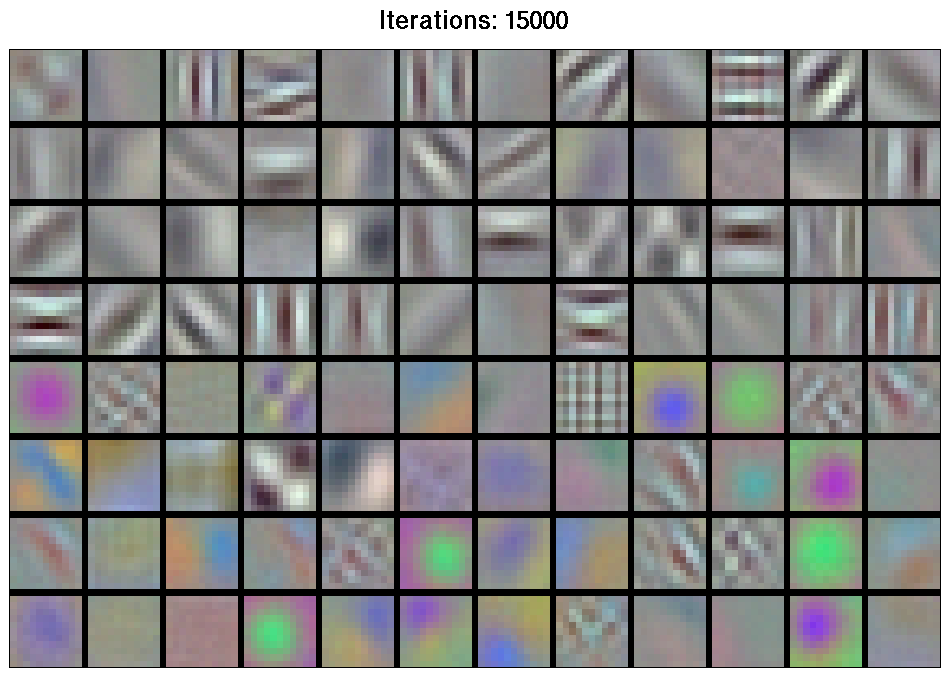
\includegraphics[scale=0.10]{images/l1_filters_iter15000.png}} \hspace{2mm}
\subfloat{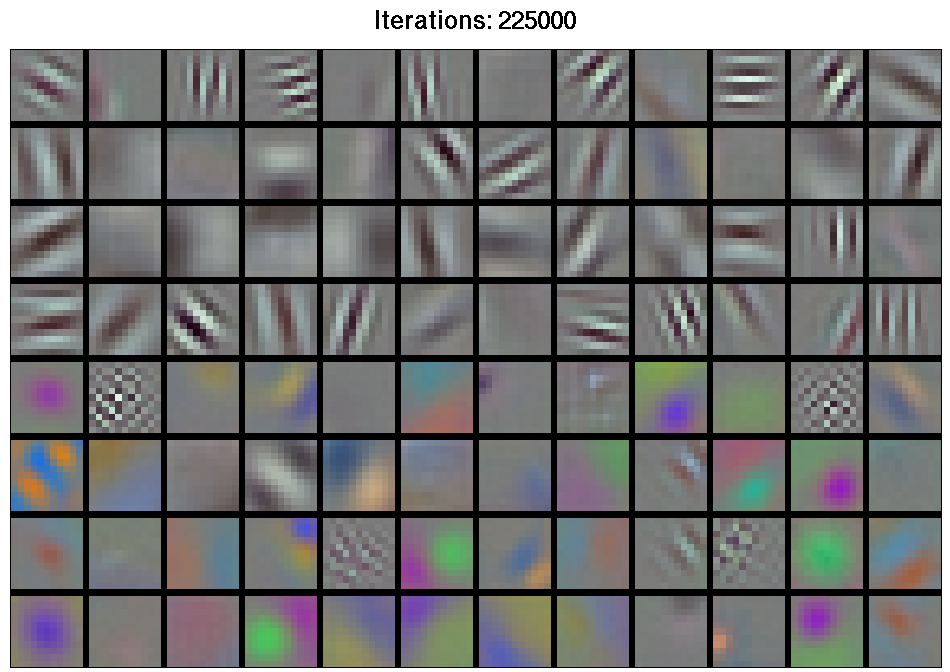
\includegraphics[scale=0.10]{images/l1_filters_iter225000.png}} \\
\subfloat{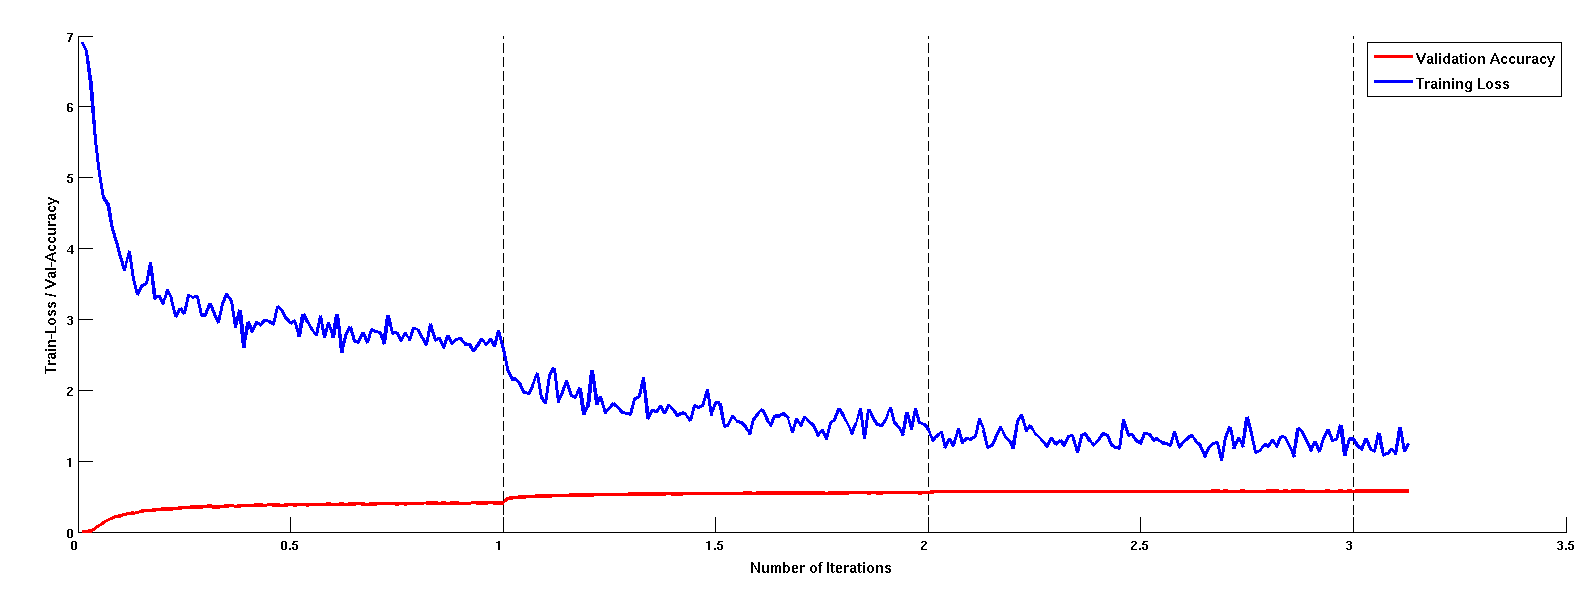
\includegraphics[scale=0.15]{images/training_loss.png}}
\caption{Evolution of Layer 1 Filters.}
\label{fig:conv1}
\end{figure}

It is quite surprising to note that by 15K iterations all layers are within 80\% and at 50K iterations within 90\% of there final performance. 
This observation raises two interesting questions. The first, is it the case that the network pretty early on in the training learn a good set parameters which are critical to generalization ?  


\setlength{\tabcolsep}{4pt}
\begin{table}
\begin{center}
\caption{Variation in classification accuracy (mean-AP) on PASCAL VOC 2007 challenge using features extracted from different layers of Alex-Net as a function of number of iterations.}
\label{table:headings}
\begin{tabular}{lcccccccc}
\hline\noalign{\smallskip}
Layer  & 5K & 15K & 25K & 35K & 45K & 95K & 105K & 310K \\
\noalign{\smallskip}
\hline
\noalign{\smallskip}
pool-1 & 23.0 & 24.3 & 24.4 & 24.5 & 24.6 & 24.8 & 24.7 & 25.1\\
pool-2 & 33.7 & 40.4 & 40.9 & 41.8 & 42.0 & 43.2 & 44.0 & 45.0\\
conv-3 & 34.2 & 46.8 & 47.0 & 48.2 & 48.5 & 49.4 & 51.6 & 50.1\\
conv-4 & 33.5 & 49.0 & 48.7 & 50.2 & 50.6 & 51.6 & 54.1 & 54.2\\
pool-5 & 33.0 & 53.4 & 55.0 & 56.8 & 57.4 & 59.2 & 63.5 & 65.6\\
relu-6 & 34.2 & 59.7 & 62.6 & 62.7 & 64.1 & 65.6 & 69.3 & 70.6\\
relu-7 & 30.9 & 61.3 & 64.1 & 65.1 & 65.8 & 67.8 & 71.8 & 73.2\\
\hline
\end{tabular}
\end{center}
\end{table}
\setlength{\tabcolsep}{1.4pt}

**Maybe-Do** Results from a n/w with only 400 units.


\setlength{\tabcolsep}{1pt}
\begin{table}
\begin{center}
\caption{What happens when we start from a network tuned only for a small number of iterations.}
\label{table:det-trajectory}
\tiny
\begin{tabular}{l|cccccccccccccccccccc||c}
\hline\noalign{\smallskip}
Feature & aero & bike & bird & boat & bottle & bus & car & cat & chair & cow & table & dog & horse & mbike & person & plant & sheep & sofa & train & tv & mAP \\
\noalign{\smallskip}
\hline
l5(50-50) & 55.2 & 58.4 & 31.0 & 28.8 & 21.0 & 53.5 & 63.6 & 41.0 & 25.4 & 44.7 & 40.9 & 34.9 & 49.5 & 56.9 & 43.8 & 25.2 & 45.3 & 31.2 & 48.7 & 54.4 & 42.7 \\
l5 (full) & 57.8 & 63.9 & 38.8 & 28.0 & 29.0&54.8&66.9&51.3 & 30.5 & 52.1 & 45.2 & 43.2 & 57.3 & 58.8 & 46.0 & 27.2 & 51.2 & 39.3 & 53.3 & 56.6 & 47.6 \\
\hline
l7(50-50) & 58.7 & 64.8 & 38.2 & 34.9 & 25.9 & 59.5 & 69.5 & 46.2 & 28.7 & 52.4 & 45.2 & 44.3 & 57.3 & 63.4 & 52.4 & 28.0 & 51.5 & 34.9 & 56.0 & 59.4 & 48.6 \\
l7(full) & 64.3 & 69.6 & 50.1 & 41.8 & 32.0 & 62.6 & 71.0 & 60.6 & 32.8 & 58.5 & 46.4 & 56.0 & 60.0 & 66.9 & 54.2 & 31.5 & 52.7 & 48.8 & 57.7 & 64.7 & 54.1 \\
\hline
\end{tabular}
\end{center}
\end{table}
\setlength{\tabcolsep}{1.4pt}

\section{What are different layers encoding ?}

\begin{frame}{Clip image}
\begin{figure}[H]
\centering
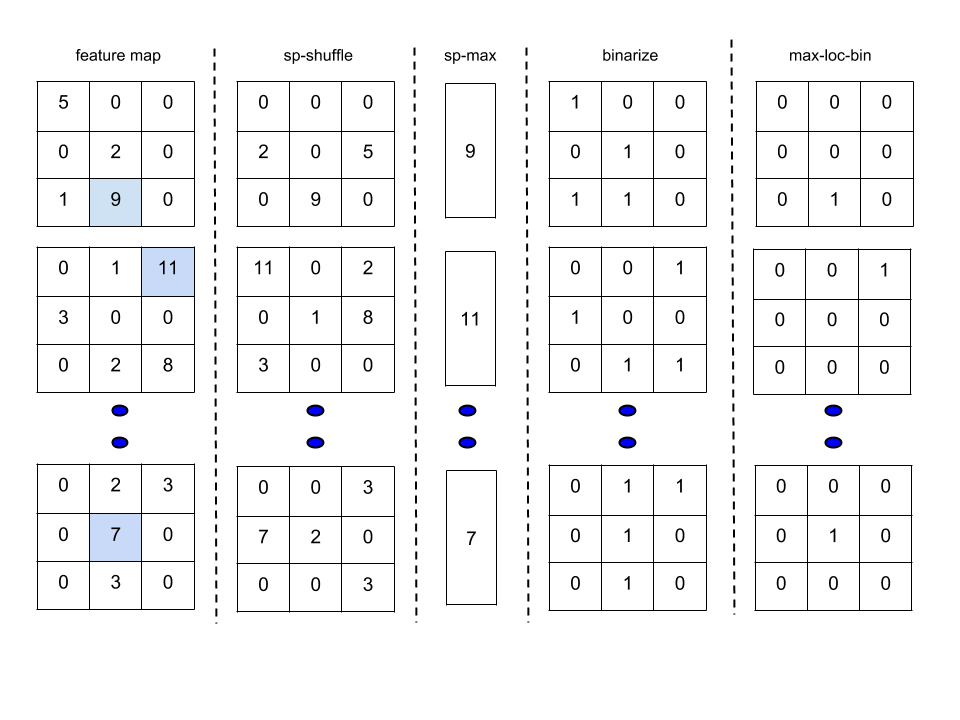
\includegraphics[height=6.5cm]{images/features.png}
\caption{Illustration of different features used in analysis described in sec. Each 3*3 block in first column is a feature map, the second column is obtained after applying an independent random  shuffle to each feature map, third column (spatial max) takes the max activation value in each featue map, fourth shows the feature vector after binarization whereas the last column selects the maximum value in each feature map and also retains its location. }
\label{fig:features}
\end{figure}
\end{frame}
\subsection{How Distributed is the Code ?}
How information is represented in deep architectures such as convolutional neural networks is an open question. On one hand, we know that the first layer learns gabor like edge detectors and that final layers have class specific units, but on the other hand we are far from understanding the nature of representations in the middle layers. Developing this understanding is crucial in order to effectively devise methods capable of fully exploiting the rich feature hierarchy provided by conv-nets.

Some recent work addressing this question has focussed on developing visualization techniques (zeiler, simoyan, google paper) to understand feature tuning of different units. Their results indicate the presence of some very specialized units tuned to certain objects such as cats and faces. Although visualizations provide interesting insights, they donot convey the full story. In particular, such results are subjective and it is often hard to draw conclusions about tuning properties of a population of units. 

From our analysis, we find that in order to predict the category of a given image, neither the magnitude nor the location of where filters activate is critical. On the other hand, 

The question we ask is whether the representation learned by conv-nets consist of many "grand-mother cells" (specifically tuned units for various classes) or whether the information is in the distributed activation of many filters. In case, there are specifically tuned units, we expect that activations of a relatively few filters should suffice for deciding the class of an image. On the other hand, in case of a distributed representation, we will need to consider activation profile of a relatively large number of filters in order to make a decision. 

As described in section .. we compute the entropy of each filter in the fifth layer of the network. Next, we rank all the filters by their entropy. At pool-5, each image produces a $6 \times 6 \times 256 $ feature vector (256 filter maps of size $6 \times 6$). For each filter map - we select the maximum activation which results into a 256-dimensional vector. Now, we train SVM 
 
For tasks of image classification, bounding box classification - position doesnot really matter. 

\subsection{How important is the magnitude of activation ?}


\subsection{How important is where a certain filter activates ?}


\setlength{\tabcolsep}{1pt}
\begin{table}
\begin{center}
\caption{Detection: Effect of various feature transformations.}
\label{table:headings}
\tiny
\begin{tabular}{l|cccccccccccccccccccc||c}
\hline\noalign{\smallskip}
Feature & aero & bike & bird & boat & bottle & bus & car & cat & chair & cow & table & dog & horse & mbike & person & plant & sheep & sofa & train & tv & mAP \\
\noalign{\smallskip}
\hline
spMax & 35.0 & 38.7 & 17.3 & 16.9 & 13.9 & 38.4 & 45.6 & 29.2 & 11.0 & 20.2 & 21.0 & 23.5 & 27.2 & 37.0 & 20.5 & 7.0 & 30.3 & 13.4 & 28.3 & 32.9 & 25.4 \\
sm-bn-lc & 49.1 & 48.0 & 19.0 & 15.2 & 12.9 & 44.7 & 57.0 & 32.8 & 11.9 & 32.5 & 19.0 & 25.0 & 37.5 & 41.6 & 34.8 & 15.6 & 34.1 & 13.0 & 35.7 & 44.9 & 31.2 \\
crop-1 & 48.2 & 59.8 & 32.2 & 20.0 & 24.6 & 46.2 & 61.2 & 41.6 & 20.6 & 46.3 & 32.9 & 38.6 & 49.9 & 53.1 & 41.8 & 25.1 & 45.0 & 23.8 & 46.2 & 51.7 & 40.4 \\
binary & 57.9 & 61.3 & 32.6 & 24.7 & 27.5 & 55.0 & 64.7 & 49.8 & 25.3 & 47.4 & 44.5 & 40.3 & 54.6 & 56.4 & 43.6 & 27.1 & 48.4 & 41.6 & 54.3 & 57.6 & 45.7 \\
pool-5  & 57.8 & 63.9 & 38.8 & 28.0 & 29.0 & 54.8 & 66.9 & 51.3 & 30.5 & 52.1 & 45.2 & 43.2 & 57.3 & 58.8 & 46.0 & 27.2 & 51.2 & 39.3 & 53.3 & 56.6 & 47.6 \\
\noalign{\smallskip}
\hline
\end{tabular}
\end{center}
\end{table}
\setlength{\tabcolsep}{1.4pt}



\setlength{\tabcolsep}{4pt}
\begin{table}
\begin{center}
\caption{Mean AP on PASCAL-VOC 2007 Classification}
\label{table:headings}
\begin{tabular}{lccccc}
\hline\noalign{\smallskip}
Layer Name & Unroll & Spatial-Shuffle & Spatial-Max & Binarize & Binarize+Loc\\
\noalign{\smallskip}
\hline
\noalign{\smallskip}
pool-1 & 25.1 & 15.0 & 19.5 & 25.4 \\
pool-2 & 44.9 & 33.5 & 40.2 & 43.0\\
conv-3 & 50.1 & 40.4 & 54.2 & 47.0\\
conv-4 & 54.2 & 45.3 & 57.0 & 51.3\\
pool-5 & 65.6 & 59.6 & 62.6 & 60.5\\
relu-6 & 70.6 &  -   &  -   & 71.4 \\
relu-7 & 73.6 &  -   &  -   & 74.1 \\
\hline
\end{tabular}
\end{center}
\end{table}
\setlength{\tabcolsep}{1.4pt}


\setlength{\tabcolsep}{4pt}
\begin{table}
\begin{center}
\caption{Comparing classification performance on ground truth boxes of a network trained on imagenet to one fine-tuned for pascal.}
\label{table:headings}
\begin{tabular}{lccccc}
\hline\noalign{\smallskip}
Layer Name & Alex-Net & Fine-Tune & Alex-Net (sp-max) & Fine-Tune (sp-max) \\
\noalign{\smallskip}
\hline
\noalign{\smallskip}
Pool-1 & 0.4321 & 0.4322 & 0.1374 & 0.1346 \\
Pool-2 & 0.6710 & 0.6770 & 0.5112 & 0.5124\\
Conv-3 & 0.7331 & 0.7368 & 0.6341 & 0.6391\\
Conv-4 & 0.7547 & 0.7782 & 0.6658 & 0.6889\\
Pool-5 & 0.7911 & 0.7951 & 0.6876 & 0.7429 \\
fc-6   & 0.7944 & 0.8232 & - & -\\
fc-7   & 0.7985 & 0.8511 & - & -\\
\hline
\end{tabular}
\end{center}
\end{table}
\setlength{\tabcolsep}{1.4pt}






\subsection {Other Stuff}
Discriminative Training - Layerwise ?
Are 4096 units required during fine-tuning or can we reduce it ?
When do the filters in the lower layers get learnt ?
Can we only have 2 layers and still learn similar filters ? - answer seems to be yes.



\section{blah}

Sparisty of different layers ? The fact that norm is really different on bounding boxes, vs images etc.

We start of by comparing performances of each 

(1) Binarizing Pool-5 features doesnt lead to much decrease in performance.

(2) Taking the max, binarizing it - but retaining its position - degrades performance substantially on detection using selective search. 

(3) The lower layers get trained pretty quickly. The training happens in almost a layer-wise manner. 


Steady growth in performance conv 1 - prob. 
We ask the question - are the neurons higher up becoming more tuned. Grand-Mother cells v/s distributed representation question! Answer this question we look into the entropy of units across layers. Since, an image in pascal-challenge can have multiple labels we focus on ground-truth bounding boxes.


\subsection{How good are individual layers?}
As a first step in our analysis, we evaluate the quality of filters extracted from each layer of our neural network for the task of image classification on PASCAL-VOC-2007. Specifically, we train a linear svm for each class. We observe a gradual increase in classification performance as we move up in the network. The results are presented in table. 

\setlength{\tabcolsep}{4pt}
\begin{table}
\begin{center}
\caption{Mean AP on PASCAL-VOC 2007 Classification}
\label{table:headings}
\begin{tabular}{lc|lc|lc|lc|lc}
\hline\noalign{\smallskip}
Layer & mAP & Layer & mAP & Layer & mAP & Layer & mAP & Layer & mAP \\
\noalign{\smallskip}
\hline
\noalign{\smallskip}
conv-1 & 22.0 & conv-2 & 42.1 & conv-3 & 50.3 & conv-5 & 62.3 & fc-7 & 74.7 \\
relu-1 & 22.1 & relu-2 & 42.0 & relu-3 & 50.1 & pool-5 & 65.6  & relu-7 & 73.6 \\ 
pool-1 & 25.1 & pool-2 & 44.9 & conv-4 & 54.2 & fc-6   & 72.1  & fc-8 & 73.4 \\
norm-1 & 34.3 & norm-2 & 46.1 & relu-4 & 54.2 & relu-6 & 70.6 & prob & 68.1 \\ 
\hline
\end{tabular}
\end{center}
\end{table}
\setlength{\tabcolsep}{1.4pt}

For the purpose of later experiments we restrict ourselves to the main 7 layers which are outputs after norm-1,norm-2,rely 

\subsection{Distributed Code v/s Tuned Units}
Method of computing entropy. 

Features from convolutional neural networks have known to generalize well to other data-sets. So, we  also want to understand the effect of fine-tuning.  

Units become more specific - but entropy of individual units - doesnt really increases until one reaches layer 6. (Ground Truth Bounding Box.) Put the picture below without the fine-tuned network.


In order to estimate the entropy, for all ground truth bounding boxes, we compute activations of each filter (both in fully-connected and convloutional layers). With each activation value we associate the class-label of the bounding box. Next, we sort the scores in decreasing order and compute entropy of the histogram counts of classes at 100 equally spaced thresholds. The area under this curve is used as a measure of entropy. 

(Contrast to mid-level patches idea - where greedily select filters based on entropy). 

\begin{figure}
\centering
\subfloat{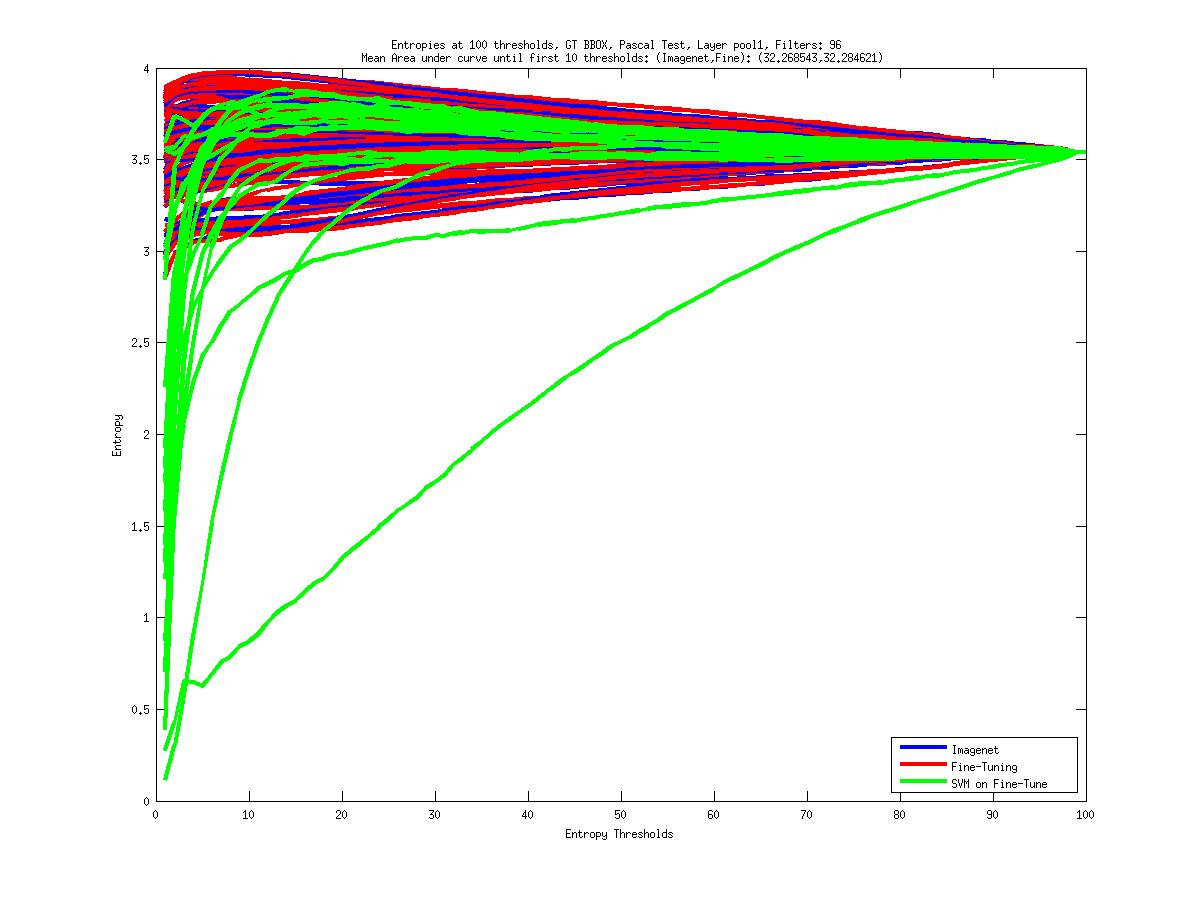
\includegraphics[scale=0.15]{images/pool1_th100_plot.jpg}}
\subfloat{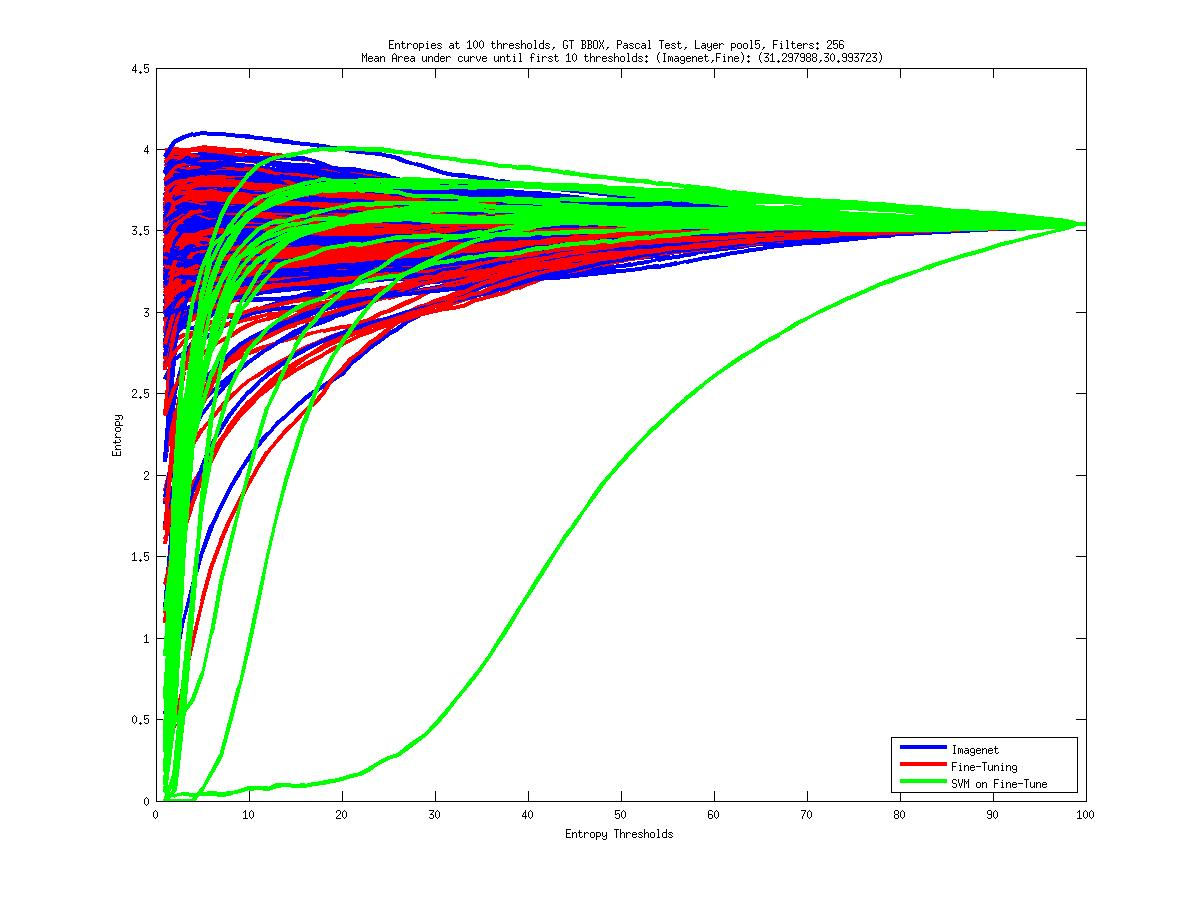
\includegraphics[scale=0.15]{images/pool5_th100_plot.jpg}} \\
\subfloat{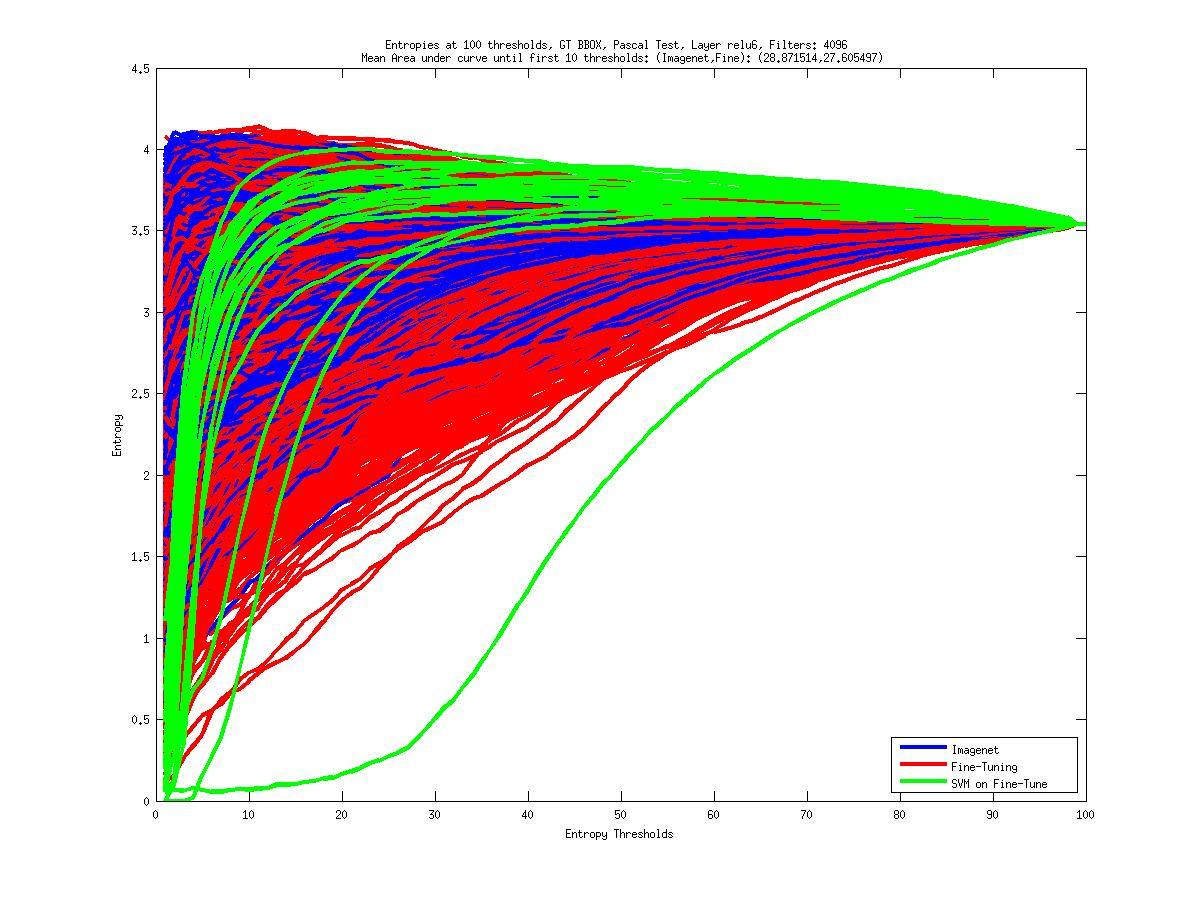
\includegraphics[scale=0.15]{images/relu6_th100_plot.jpg}} 
\subfloat{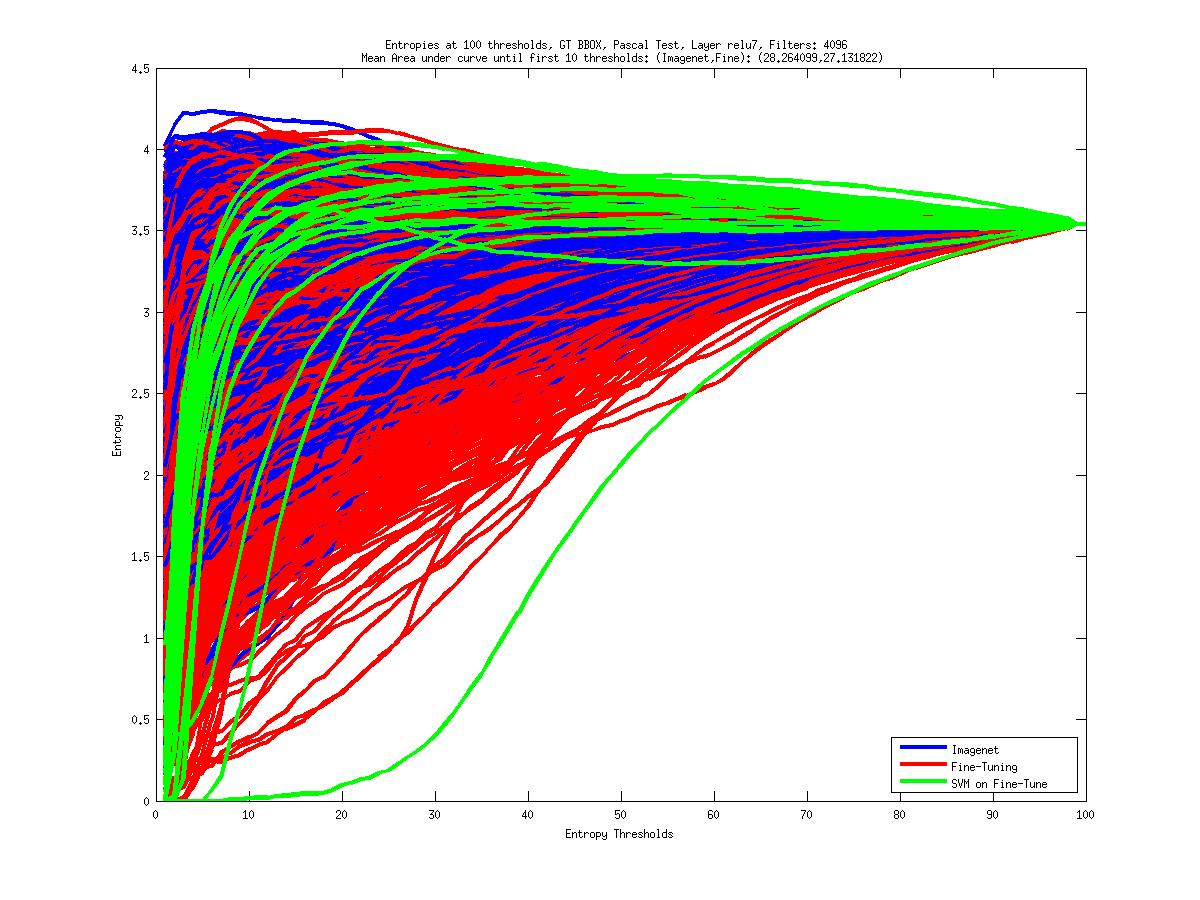
\includegraphics[scale=0.15]{images/relu7_th100_plot.jpg}}
\caption{Entropy filters at various layers.}
\label{fig:example}
\end{figure}


\begin{figure}[H]
\centering
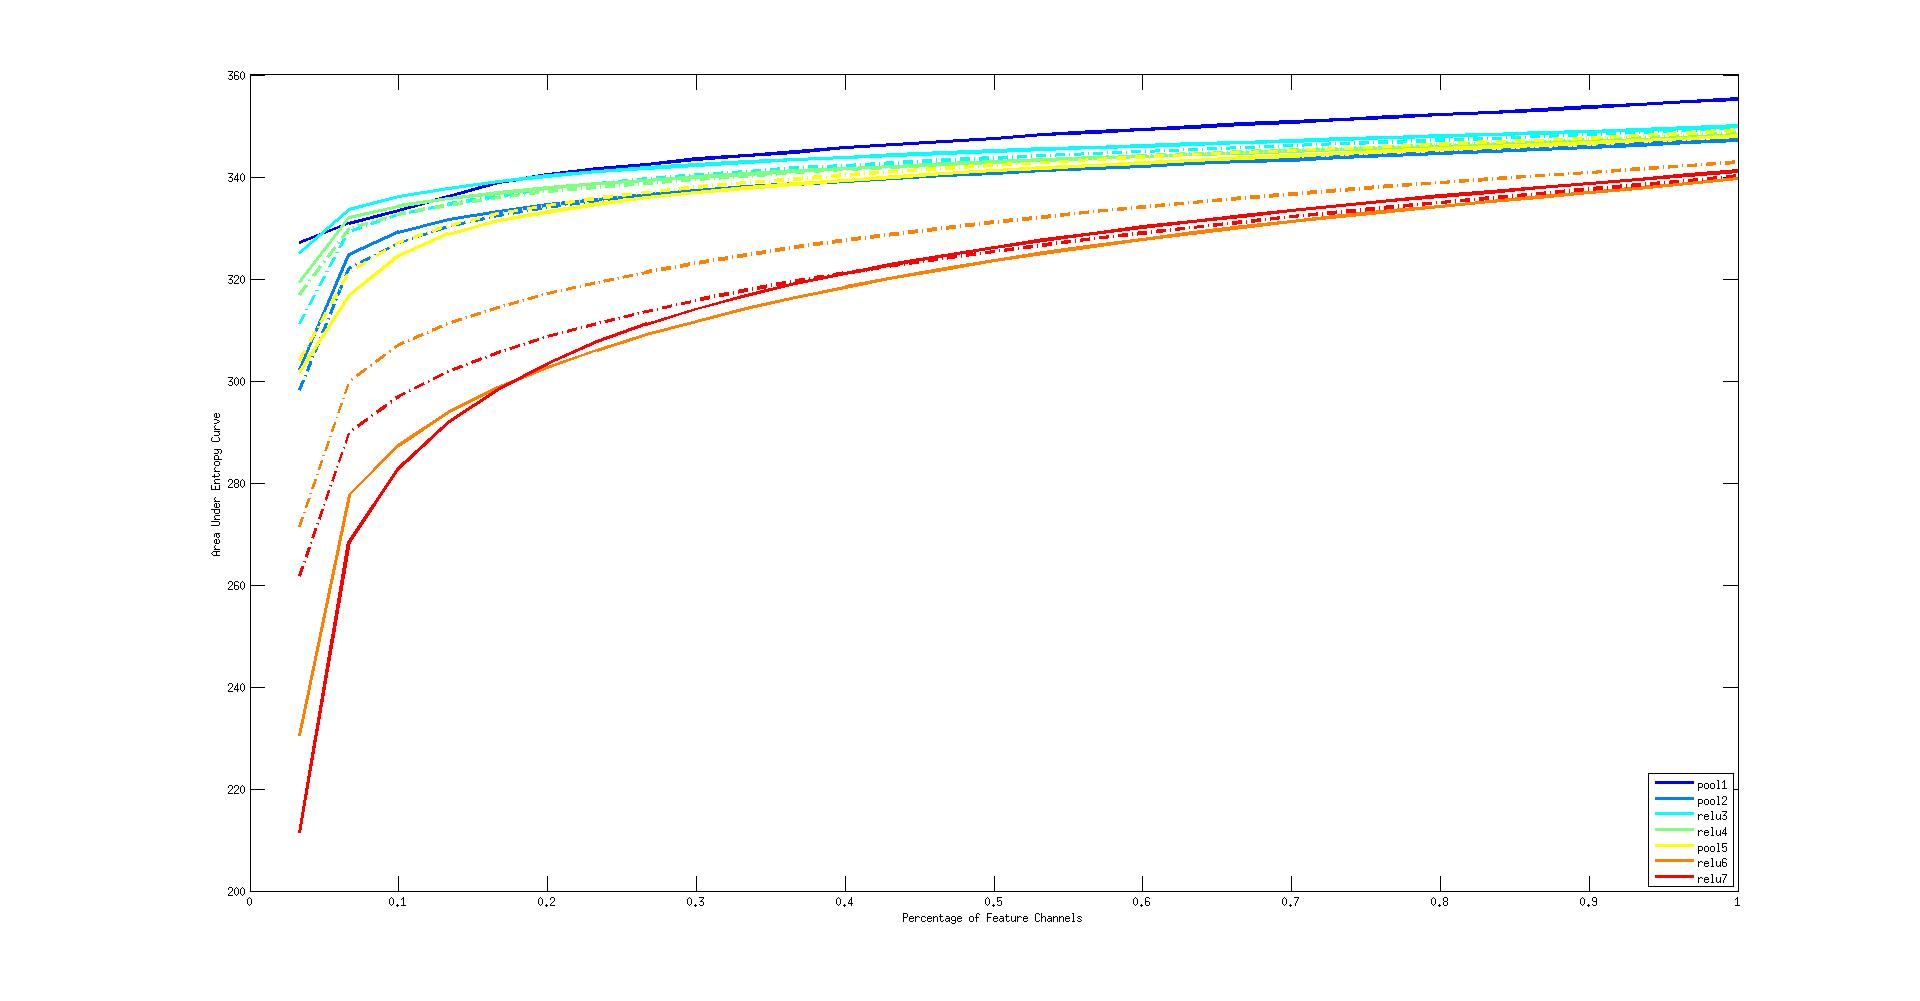
\includegraphics[height=6.5cm]{images/entropy_layers.jpg}
\caption{The plot shows the variation in entropy of different layers of a convolutional network trained on imagenet (dot-dash line) and a network fine-tuned for object detection on PASCAL dataset.}
\label{fig:example}
\end{figure}

\begin{figure}
\centering
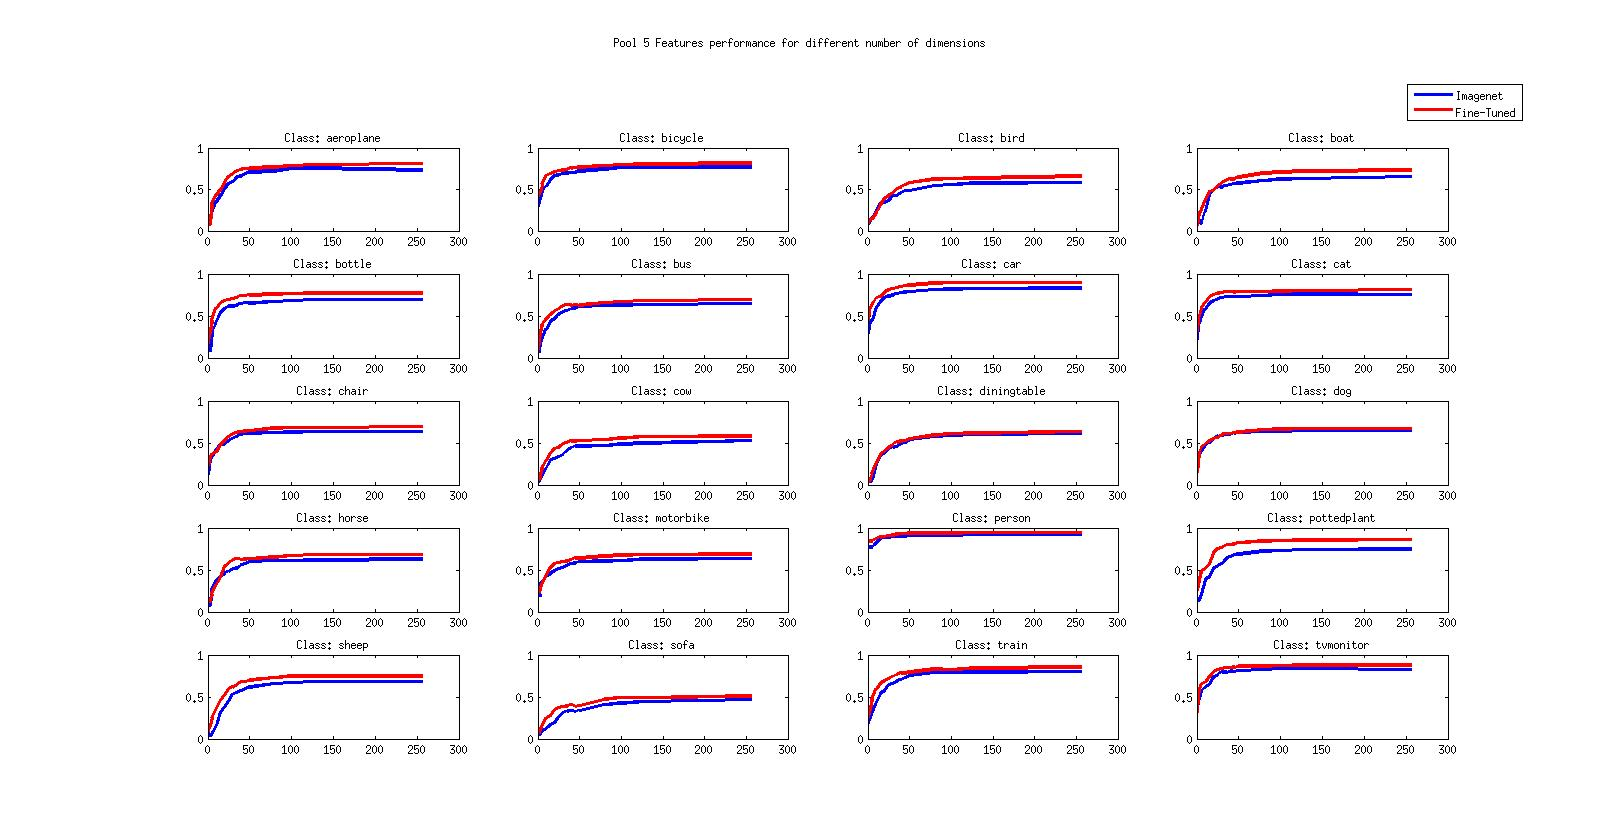
\includegraphics[height=6.5cm]{images//pool5_bbox_seldims.jpeg}
\caption{Number of useful dimensions based on the spatial max criterion. (GT-BBOX Classification - Fine Tuned N/W)}
\label{fig:example}
\end{figure}










\section{Conclusions and Open-Challenges}

The paper ends with a conclusion. 


\clearpage\mbox{}Page \thepage\ of the manuscript.
\clearpage\mbox{}Page \thepage\ of the manuscript.
\clearpage\mbox{}Page \thepage\ of the manuscript.
\clearpage\mbox{}Page \thepage\ of the manuscript.
\clearpage\mbox{}Page \thepage\ of the manuscript.
\clearpage\mbox{}Page \thepage\ of the manuscript.
\clearpage\mbox{}Page \thepage\ of the manuscript.
This is the last page of the manuscript.
\par\vfill\par
Now we have reached the maximum size of the ECCV 2014 submission (excluding references).
References should start immediately after the main text, but can continue on p.15 if needed.

\clearpage

\bibliographystyle{splncs}
\bibliography{egbib}
\end{document}
